\documentclass[aspectratio=169]{beamer}

\usetheme{Boadilla}
\usefonttheme{professionalfonts}
\setbeamertemplate{navigation symbols}{}
\setbeamertemplate{itemize items}[circle]
\setbeamertemplate{enumerate items}[default]
\setbeamertemplate{headline}{}

\usepackage[utf8]{inputenc}
\usepackage[T1]{fontenc}
\usepackage{lmodern}
\usepackage{amsmath}
\usepackage{booktabs}
\usepackage{tabularx}
\usepackage{array}
\usepackage{hyperref}
\usepackage[strings]{underscore}
\usepackage{listings}
\usepackage{tikz}
\usetikzlibrary{arrows.meta,positioning,fit,calc,shapes.geometric}
\usepackage{xcolor}

\definecolor{courseblue}{HTML}{12355B}
\definecolor{coursegold}{HTML}{C98A2E}
\definecolor{courseice}{HTML}{EEF3F8}
\definecolor{coursegreen}{HTML}{2F6B4F}
\definecolor{coursegray}{HTML}{4B5563}
\definecolor{codebg}{HTML}{F7F9FC}
\definecolor{codecomment}{HTML}{5E6C84}
\definecolor{codestring}{HTML}{0B6E4F}

\setbeamercolor{palette primary}{bg=courseblue,fg=white}
\setbeamercolor{palette secondary}{bg=coursegold,fg=white}
\setbeamercolor{palette tertiary}{bg=courseblue,fg=white}
\setbeamercolor{palette quaternary}{bg=coursegold,fg=white}
\setbeamercolor{structure}{fg=courseblue}
\setbeamercolor{frametitle}{bg=courseice,fg=courseblue}
\setbeamercolor{title}{fg=courseblue}
\setbeamercolor{block title}{bg=courseblue,fg=white}
\setbeamercolor{block body}{bg=courseice,fg=black}
\setbeamercolor{normal text}{fg=black,bg=white}
\setbeamercolor{alerted text}{fg=coursegold}

\setbeamerfont{footline}{size=\scriptsize}

\setbeamertemplate{footline}{
  \leavevmode
  \hbox{
    \begin{beamercolorbox}[wd=.33\paperwidth,ht=2.8ex,dp=1.2ex,leftskip=0.8em]{palette primary}%
      University of Trieste
    \end{beamercolorbox}%
    \begin{beamercolorbox}[wd=.49\paperwidth,ht=2.8ex,dp=1.2ex,center]{palette tertiary}%
      \coursename{} \textbar{} \coursecode
    \end{beamercolorbox}%
    \begin{beamercolorbox}[wd=.18\paperwidth,ht=2.8ex,dp=1.2ex,rightskip=0.8em plus1fil]{palette secondary}%
      \insertframenumber{} / \inserttotalframenumber
    \end{beamercolorbox}%
  }
}

\hypersetup{
  colorlinks=true,
  linkcolor=courseblue,
  urlcolor=coursegreen
}

\lstdefinestyle{coursepython}{
  language=Python,
  basicstyle=\ttfamily\footnotesize,
  keywordstyle=\color{courseblue}\bfseries,
  commentstyle=\color{codecomment}\itshape,
  stringstyle=\color{codestring},
  showstringspaces=false,
  columns=fullflexible,
  keepspaces=true,
  frame=single,
  framerule=0.6pt,
  rulecolor=\color{courseblue},
  backgroundcolor=\color{codebg},
  xleftmargin=0.4em,
  xrightmargin=0.4em,
  aboveskip=0.4em,
  belowskip=0.2em
}

\newcommand{\coursename}{Data-driven Systems Engineering}
\newcommand{\coursecode}{440MI / 305SM}
\newcommand{\coursefooter}{}

\newcommand{\learninggoals}[1]{
  \begin{block}{Learning goals}
  #1
  \end{block}
}

\newcommand{\repoactivity}[1]{
  \begin{block}{Repo activity}
  #1
  \end{block}
}

\newcommand{\readinglist}[1]{
  \begin{block}{Papers and materials}
  {\footnotesize #1}
  \end{block}
}

\newcommand{\coursecontextframe}[5]{
  \begin{frame}{Course Map and Running Cases}
  \centering
  \begin{tikzpicture}[node distance=0.28cm]
  \node[flowbox, minimum width=1.45cm, minimum height=0.8cm] (problem) {\scriptsize Problem};
  \node[flowbox, minimum width=1.45cm, minimum height=0.8cm, right=of problem] (data) {\scriptsize Data};
  \node[flowbox, minimum width=1.45cm, minimum height=0.8cm, right=of data] (features) {\scriptsize Features};
  \node[flowbox, minimum width=1.45cm, minimum height=0.8cm, right=of features] (model) {\scriptsize Model};
  \node[flowbox, minimum width=1.45cm, minimum height=0.8cm, right=of model] (interface) {\scriptsize Interface};
  \node[flowbox, minimum width=1.45cm, minimum height=0.8cm, right=of interface] (delivery) {\scriptsize Delivery};
  \node[flowbox, minimum width=1.45cm, minimum height=0.8cm, right=of delivery] (monitor) {\scriptsize Monitor};
  \node[accentbox, minimum width=1.6cm, minimum height=0.8cm, right=of monitor] (evolution) {\scriptsize Evolution};
  \foreach \a/\b in {problem/data,data/features,features/model,model/interface,interface/delivery,delivery/monitor,monitor/evolution} {
    \draw[arrow] (\a) -- (\b);
  }
  \end{tikzpicture}

  \vspace{0.5em}
  \begin{block}{Today in the course}
  \textbf{Focus:} #1

  \textbf{Bridge:} #2
  \end{block}

  \begin{columns}[T]
  \column{0.48\textwidth}
  \begin{block}{Fraud case}
  {\footnotesize #3}
  \end{block}
  \column{0.48\textwidth}
  \begin{block}{Pasteurization case}
  {\footnotesize #4}
  \end{block}
  \end{columns}

  \vspace{0.3em}
  {\footnotesize \textbf{Course thread:} #5}
  \coursefooter
  \end{frame}
}

\newcommand{\classclosingframe}[4]{
  \begin{frame}{From This Class to the Next}
  \begin{block}{What stays with us}
  #1
  \end{block}

  \begin{columns}[T]
  \column{0.48\textwidth}
  \begin{block}{Project use}
  {\footnotesize #2}
  \end{block}
  \column{0.48\textwidth}
  \begin{block}{Next connection}
  {\footnotesize #3}
  \end{block}
  \end{columns}

  \vspace{0.3em}
  {\footnotesize \textbf{Course thread:} #4}
  \coursefooter
  \end{frame}
}

\tikzset{
  flowbox/.style={
    rounded corners=3pt,
    draw=courseblue,
    fill=courseice,
    very thick,
    minimum width=2.2cm,
    minimum height=0.9cm,
    align=center,
    font=\small
  },
  accentbox/.style={
    rounded corners=3pt,
    draw=coursegold,
    fill=coursegold!15,
    very thick,
    minimum width=2.2cm,
    minimum height=0.9cm,
    align=center,
    font=\small
  },
  arrow/.style={
    -{Latex[length=2.5mm,width=2mm]},
    thick,
    draw=courseblue
  }
}

% Visual layer on top of common.tex: tiles, icons, a progress-strip section divider, and a footer
% strip that defines the concepts appearing for the first time on each slide.
% Same look as the Class 20 deck. Load with:  \documentclass[aspectratio=169]{beamer}

\usetheme{Boadilla}
\usefonttheme{professionalfonts}
\setbeamertemplate{navigation symbols}{}
\setbeamertemplate{itemize items}[circle]
\setbeamertemplate{enumerate items}[default]
\setbeamertemplate{headline}{}

\usepackage[utf8]{inputenc}
\usepackage[T1]{fontenc}
\usepackage{lmodern}
\usepackage{amsmath}
\usepackage{booktabs}
\usepackage{tabularx}
\usepackage{array}
\usepackage{hyperref}
\usepackage[strings]{underscore}
\usepackage{listings}
\usepackage{tikz}
\usetikzlibrary{arrows.meta,positioning,fit,calc,shapes.geometric}
\usepackage{xcolor}

\definecolor{courseblue}{HTML}{12355B}
\definecolor{coursegold}{HTML}{C98A2E}
\definecolor{courseice}{HTML}{EEF3F8}
\definecolor{coursegreen}{HTML}{2F6B4F}
\definecolor{coursegray}{HTML}{4B5563}
\definecolor{codebg}{HTML}{F7F9FC}
\definecolor{codecomment}{HTML}{5E6C84}
\definecolor{codestring}{HTML}{0B6E4F}

\setbeamercolor{palette primary}{bg=courseblue,fg=white}
\setbeamercolor{palette secondary}{bg=coursegold,fg=white}
\setbeamercolor{palette tertiary}{bg=courseblue,fg=white}
\setbeamercolor{palette quaternary}{bg=coursegold,fg=white}
\setbeamercolor{structure}{fg=courseblue}
\setbeamercolor{frametitle}{bg=courseice,fg=courseblue}
\setbeamercolor{title}{fg=courseblue}
\setbeamercolor{block title}{bg=courseblue,fg=white}
\setbeamercolor{block body}{bg=courseice,fg=black}
\setbeamercolor{normal text}{fg=black,bg=white}
\setbeamercolor{alerted text}{fg=coursegold}

\setbeamerfont{footline}{size=\scriptsize}

\setbeamertemplate{footline}{
  \leavevmode
  \hbox{
    \begin{beamercolorbox}[wd=.33\paperwidth,ht=2.8ex,dp=1.2ex,leftskip=0.8em]{palette primary}%
      University of Trieste
    \end{beamercolorbox}%
    \begin{beamercolorbox}[wd=.49\paperwidth,ht=2.8ex,dp=1.2ex,center]{palette tertiary}%
      \coursename{} \textbar{} \coursecode
    \end{beamercolorbox}%
    \begin{beamercolorbox}[wd=.18\paperwidth,ht=2.8ex,dp=1.2ex,rightskip=0.8em plus1fil]{palette secondary}%
      \insertframenumber{} / \inserttotalframenumber
    \end{beamercolorbox}%
  }
}

\hypersetup{
  colorlinks=true,
  linkcolor=courseblue,
  urlcolor=coursegreen
}

\lstdefinestyle{coursepython}{
  language=Python,
  basicstyle=\ttfamily\footnotesize,
  keywordstyle=\color{courseblue}\bfseries,
  commentstyle=\color{codecomment}\itshape,
  stringstyle=\color{codestring},
  showstringspaces=false,
  columns=fullflexible,
  keepspaces=true,
  frame=single,
  framerule=0.6pt,
  rulecolor=\color{courseblue},
  backgroundcolor=\color{codebg},
  xleftmargin=0.4em,
  xrightmargin=0.4em,
  aboveskip=0.4em,
  belowskip=0.2em
}

\newcommand{\coursename}{Data-driven Systems Engineering}
\newcommand{\coursecode}{440MI / 305SM}
\newcommand{\coursefooter}{}

\newcommand{\learninggoals}[1]{
  \begin{block}{Learning goals}
  #1
  \end{block}
}

\newcommand{\repoactivity}[1]{
  \begin{block}{Repo activity}
  #1
  \end{block}
}

\newcommand{\readinglist}[1]{
  \begin{block}{Papers and materials}
  {\footnotesize #1}
  \end{block}
}

\newcommand{\coursecontextframe}[5]{
  \begin{frame}{Course Map and Running Cases}
  \centering
  \begin{tikzpicture}[node distance=0.28cm]
  \node[flowbox, minimum width=1.45cm, minimum height=0.8cm] (problem) {\scriptsize Problem};
  \node[flowbox, minimum width=1.45cm, minimum height=0.8cm, right=of problem] (data) {\scriptsize Data};
  \node[flowbox, minimum width=1.45cm, minimum height=0.8cm, right=of data] (features) {\scriptsize Features};
  \node[flowbox, minimum width=1.45cm, minimum height=0.8cm, right=of features] (model) {\scriptsize Model};
  \node[flowbox, minimum width=1.45cm, minimum height=0.8cm, right=of model] (interface) {\scriptsize Interface};
  \node[flowbox, minimum width=1.45cm, minimum height=0.8cm, right=of interface] (delivery) {\scriptsize Delivery};
  \node[flowbox, minimum width=1.45cm, minimum height=0.8cm, right=of delivery] (monitor) {\scriptsize Monitor};
  \node[accentbox, minimum width=1.6cm, minimum height=0.8cm, right=of monitor] (evolution) {\scriptsize Evolution};
  \foreach \a/\b in {problem/data,data/features,features/model,model/interface,interface/delivery,delivery/monitor,monitor/evolution} {
    \draw[arrow] (\a) -- (\b);
  }
  \end{tikzpicture}

  \vspace{0.5em}
  \begin{block}{Today in the course}
  \textbf{Focus:} #1

  \textbf{Bridge:} #2
  \end{block}

  \begin{columns}[T]
  \column{0.48\textwidth}
  \begin{block}{Fraud case}
  {\footnotesize #3}
  \end{block}
  \column{0.48\textwidth}
  \begin{block}{Pasteurization case}
  {\footnotesize #4}
  \end{block}
  \end{columns}

  \vspace{0.3em}
  {\footnotesize \textbf{Course thread:} #5}
  \coursefooter
  \end{frame}
}

\newcommand{\classclosingframe}[4]{
  \begin{frame}{From This Class to the Next}
  \begin{block}{What stays with us}
  #1
  \end{block}

  \begin{columns}[T]
  \column{0.48\textwidth}
  \begin{block}{Project use}
  {\footnotesize #2}
  \end{block}
  \column{0.48\textwidth}
  \begin{block}{Next connection}
  {\footnotesize #3}
  \end{block}
  \end{columns}

  \vspace{0.3em}
  {\footnotesize \textbf{Course thread:} #4}
  \coursefooter
  \end{frame}
}

\tikzset{
  flowbox/.style={
    rounded corners=3pt,
    draw=courseblue,
    fill=courseice,
    very thick,
    minimum width=2.2cm,
    minimum height=0.9cm,
    align=center,
    font=\small
  },
  accentbox/.style={
    rounded corners=3pt,
    draw=coursegold,
    fill=coursegold!15,
    very thick,
    minimum width=2.2cm,
    minimum height=0.9cm,
    align=center,
    font=\small
  },
  arrow/.style={
    -{Latex[length=2.5mm,width=2mm]},
    thick,
    draw=courseblue
  }
}
  % Visual layer on top of common.tex: tiles, icons, a progress-strip section divider, and a footer
% strip that defines the concepts appearing for the first time on each slide.
% Same look as the Class 20 deck. Load with:  \documentclass[aspectratio=169]{beamer}

\usetheme{Boadilla}
\usefonttheme{professionalfonts}
\setbeamertemplate{navigation symbols}{}
\setbeamertemplate{itemize items}[circle]
\setbeamertemplate{enumerate items}[default]
\setbeamertemplate{headline}{}

\usepackage[utf8]{inputenc}
\usepackage[T1]{fontenc}
\usepackage{lmodern}
\usepackage{amsmath}
\usepackage{booktabs}
\usepackage{tabularx}
\usepackage{array}
\usepackage{hyperref}
\usepackage[strings]{underscore}
\usepackage{listings}
\usepackage{tikz}
\usetikzlibrary{arrows.meta,positioning,fit,calc,shapes.geometric}
\usepackage{xcolor}

\definecolor{courseblue}{HTML}{12355B}
\definecolor{coursegold}{HTML}{C98A2E}
\definecolor{courseice}{HTML}{EEF3F8}
\definecolor{coursegreen}{HTML}{2F6B4F}
\definecolor{coursegray}{HTML}{4B5563}
\definecolor{codebg}{HTML}{F7F9FC}
\definecolor{codecomment}{HTML}{5E6C84}
\definecolor{codestring}{HTML}{0B6E4F}

\setbeamercolor{palette primary}{bg=courseblue,fg=white}
\setbeamercolor{palette secondary}{bg=coursegold,fg=white}
\setbeamercolor{palette tertiary}{bg=courseblue,fg=white}
\setbeamercolor{palette quaternary}{bg=coursegold,fg=white}
\setbeamercolor{structure}{fg=courseblue}
\setbeamercolor{frametitle}{bg=courseice,fg=courseblue}
\setbeamercolor{title}{fg=courseblue}
\setbeamercolor{block title}{bg=courseblue,fg=white}
\setbeamercolor{block body}{bg=courseice,fg=black}
\setbeamercolor{normal text}{fg=black,bg=white}
\setbeamercolor{alerted text}{fg=coursegold}

\setbeamerfont{footline}{size=\scriptsize}

\setbeamertemplate{footline}{
  \leavevmode
  \hbox{
    \begin{beamercolorbox}[wd=.33\paperwidth,ht=2.8ex,dp=1.2ex,leftskip=0.8em]{palette primary}%
      University of Trieste
    \end{beamercolorbox}%
    \begin{beamercolorbox}[wd=.49\paperwidth,ht=2.8ex,dp=1.2ex,center]{palette tertiary}%
      \coursename{} \textbar{} \coursecode
    \end{beamercolorbox}%
    \begin{beamercolorbox}[wd=.18\paperwidth,ht=2.8ex,dp=1.2ex,rightskip=0.8em plus1fil]{palette secondary}%
      \insertframenumber{} / \inserttotalframenumber
    \end{beamercolorbox}%
  }
}

\hypersetup{
  colorlinks=true,
  linkcolor=courseblue,
  urlcolor=coursegreen
}

\lstdefinestyle{coursepython}{
  language=Python,
  basicstyle=\ttfamily\footnotesize,
  keywordstyle=\color{courseblue}\bfseries,
  commentstyle=\color{codecomment}\itshape,
  stringstyle=\color{codestring},
  showstringspaces=false,
  columns=fullflexible,
  keepspaces=true,
  frame=single,
  framerule=0.6pt,
  rulecolor=\color{courseblue},
  backgroundcolor=\color{codebg},
  xleftmargin=0.4em,
  xrightmargin=0.4em,
  aboveskip=0.4em,
  belowskip=0.2em
}

\newcommand{\coursename}{Data-driven Systems Engineering}
\newcommand{\coursecode}{440MI / 305SM}
\newcommand{\coursefooter}{}

\newcommand{\learninggoals}[1]{
  \begin{block}{Learning goals}
  #1
  \end{block}
}

\newcommand{\repoactivity}[1]{
  \begin{block}{Repo activity}
  #1
  \end{block}
}

\newcommand{\readinglist}[1]{
  \begin{block}{Papers and materials}
  {\footnotesize #1}
  \end{block}
}

\newcommand{\coursecontextframe}[5]{
  \begin{frame}{Course Map and Running Cases}
  \centering
  \begin{tikzpicture}[node distance=0.28cm]
  \node[flowbox, minimum width=1.45cm, minimum height=0.8cm] (problem) {\scriptsize Problem};
  \node[flowbox, minimum width=1.45cm, minimum height=0.8cm, right=of problem] (data) {\scriptsize Data};
  \node[flowbox, minimum width=1.45cm, minimum height=0.8cm, right=of data] (features) {\scriptsize Features};
  \node[flowbox, minimum width=1.45cm, minimum height=0.8cm, right=of features] (model) {\scriptsize Model};
  \node[flowbox, minimum width=1.45cm, minimum height=0.8cm, right=of model] (interface) {\scriptsize Interface};
  \node[flowbox, minimum width=1.45cm, minimum height=0.8cm, right=of interface] (delivery) {\scriptsize Delivery};
  \node[flowbox, minimum width=1.45cm, minimum height=0.8cm, right=of delivery] (monitor) {\scriptsize Monitor};
  \node[accentbox, minimum width=1.6cm, minimum height=0.8cm, right=of monitor] (evolution) {\scriptsize Evolution};
  \foreach \a/\b in {problem/data,data/features,features/model,model/interface,interface/delivery,delivery/monitor,monitor/evolution} {
    \draw[arrow] (\a) -- (\b);
  }
  \end{tikzpicture}

  \vspace{0.5em}
  \begin{block}{Today in the course}
  \textbf{Focus:} #1

  \textbf{Bridge:} #2
  \end{block}

  \begin{columns}[T]
  \column{0.48\textwidth}
  \begin{block}{Fraud case}
  {\footnotesize #3}
  \end{block}
  \column{0.48\textwidth}
  \begin{block}{Pasteurization case}
  {\footnotesize #4}
  \end{block}
  \end{columns}

  \vspace{0.3em}
  {\footnotesize \textbf{Course thread:} #5}
  \coursefooter
  \end{frame}
}

\newcommand{\classclosingframe}[4]{
  \begin{frame}{From This Class to the Next}
  \begin{block}{What stays with us}
  #1
  \end{block}

  \begin{columns}[T]
  \column{0.48\textwidth}
  \begin{block}{Project use}
  {\footnotesize #2}
  \end{block}
  \column{0.48\textwidth}
  \begin{block}{Next connection}
  {\footnotesize #3}
  \end{block}
  \end{columns}

  \vspace{0.3em}
  {\footnotesize \textbf{Course thread:} #4}
  \coursefooter
  \end{frame}
}

\tikzset{
  flowbox/.style={
    rounded corners=3pt,
    draw=courseblue,
    fill=courseice,
    very thick,
    minimum width=2.2cm,
    minimum height=0.9cm,
    align=center,
    font=\small
  },
  accentbox/.style={
    rounded corners=3pt,
    draw=coursegold,
    fill=coursegold!15,
    very thick,
    minimum width=2.2cm,
    minimum height=0.9cm,
    align=center,
    font=\small
  },
  arrow/.style={
    -{Latex[length=2.5mm,width=2mm]},
    thick,
    draw=courseblue
  }
}
  % Visual layer on top of common.tex: tiles, icons, a progress-strip section divider, and a footer
% strip that defines the concepts appearing for the first time on each slide.
% Same look as the Class 20 deck. Load with:  \input{common}  \input{common_visual}
%
% Before the first \sectiondivider, a deck must define
%   \sectioncount   the number of sections, e.g. 4
%   \sectionlabels  a \foreach list of number/label pairs, e.g. 1/Need,2/Testable,3/Manage,4/Practice
% Icons come from the fontawesome5 package (Font Awesome 5 Free), e.g. \faIcon{robot}.

\usepackage{colortbl}
\usepackage{fontawesome5}
\usetikzlibrary{backgrounds}

% Slides read better without automatic hyphenation.
\hyphenpenalty=10000
\exhyphenpenalty=10000

\definecolor{coursered}{HTML}{A23B2A}
\newcommand{\goldink}{\color{coursegold!65!black}}

\tikzset{
  tile/.style={rounded corners=4pt, fill=courseice, draw=none, align=center, font=\footnotesize, inner sep=5pt},
  tileblue/.style={tile, fill=white, draw=courseblue!55, thick},
  tilegold/.style={tile, fill=coursegold!14, draw=coursegold, thick},
  tilegreen/.style={tile, fill=coursegreen!10, draw=coursegreen!70, thick},
  tilered/.style={tile, fill=coursered!8, draw=coursered!70, thick},
  tilegray/.style={tile, fill=white, draw=coursegray!55, thick, dashed},
  tag/.style={rounded corners=2pt, fill=coursegold, text=white, font=\bfseries\tiny, inner sep=2.5pt},
  chip/.style={rounded corners=3pt, fill=courseblue, text=white, font=\footnotesize\bfseries, align=center, inner sep=4pt},
  note/.style={font=\scriptsize, text=coursegray, align=left},
  arrowgold/.style={-{Latex[length=2.5mm,width=2mm]}, thick, draw=coursegold},
  arrowred/.style={-{Latex[length=2.5mm,width=2mm]}, thick, draw=coursered},
  arrowgreen/.style={-{Latex[length=2.5mm,width=2mm]}, thick, draw=coursegreen},
  arrowgray/.style={-{Latex[length=2mm,width=1.6mm]}, thick, draw=coursegray!70},
}

% A round icon badge, drawn inside a tikzpicture: x y colour icon
\newcommand{\badge}[4]{%
  \node[circle, fill=#3, text=white, minimum size=0.85cm, inner sep=0pt] at (#1,#2) {\large\faIcon{#4}};
}

% Inline tags for the kind of requirement.
\newcommand{\Ftag}{\colorbox{courseblue}{\color{white}\bfseries\scriptsize\ \ F\ \ }}
\newcommand{\NFtag}{\colorbox{coursegold}{\color{white}\bfseries\scriptsize\ NF\ }}
\newcommand{\Dtag}{\colorbox{coursegreen}{\color{white}\bfseries\scriptsize\ \ D\ \ }}
\newcommand{\MLtag}{\colorbox{coursered}{\color{white}\bfseries\scriptsize\ ML\ }}

% Footer: a strip with the concepts that appear for the first time on the slide, above the
% usual bar. The bar total counts only the main lecture; a backup slide is numbered separately.
\makeatletter
\def\conceptstext{}
\def\currentsectionname{}
\setbeamercolor{conceptbar}{bg=coursegold!12,fg=black}
\newcommand{\cterm}[2]{{\bfseries\color{courseblue}#1:}\ #2\hspace{0.8em}}
\newcommand{\newtag}{\colorbox{coursegold}{\color{white}\bfseries\tiny\ NEW\ }\hspace{0.6em}}
\setbeamertemplate{footline}{
  \leavevmode
  \vbox{%
    \ifx\conceptstext\empty\else
      \hbox{\color{coursegold}\rule{\paperwidth}{0.8pt}}%
      \hbox{\begin{beamercolorbox}[wd=\paperwidth,leftskip=0.5cm,rightskip=0.5cm,sep=3pt]{conceptbar}\scriptsize\newtag\conceptstext\end{beamercolorbox}}%
    \fi
    \hbox{%
      \begin{beamercolorbox}[wd=.33\paperwidth,ht=2.8ex,dp=1.2ex,leftskip=0.8em]{palette primary}%
        \ifbeamer@inappendix Backup\else\ifnum\value{section}>0 \arabic{section}\ \textbar\ \currentsectionname\else University of Trieste\fi\fi
      \end{beamercolorbox}%
      \begin{beamercolorbox}[wd=.49\paperwidth,ht=2.8ex,dp=1.2ex,center]{palette tertiary}%
        \coursename{} \textbar{} \coursecode
      \end{beamercolorbox}%
      \begin{beamercolorbox}[wd=.18\paperwidth,ht=2.8ex,dp=1.2ex,right,rightskip=0.8em]{palette secondary}%
        \ifbeamer@inappendix Backup \insertframenumberinappendix\else\insertframenumber{} / \insertmainframenumber\fi
      \end{beamercolorbox}%
    }}}
\makeatother
\newenvironment{cframe}[2]{\gdef\conceptstext{#2}\begin{frame}{#1}}{\end{frame}\gdef\conceptstext{}}

% Section divider: progress strip, recap of the previous part, and the roadmap of the next one.
% Arguments: number, title, icon, previously, items.
\newcommand{\sectiondivider}[5]{%
  \section{#2}\gdef\currentsectionname{#2}
  \begin{frame}
  \centering
  \begin{tikzpicture}
  \pgfmathsetmacro{\chipw}{13.6/\sectioncount}
  \foreach \i/\lab in \sectionlabels {
    \ifnum\i<#1 \def\chipfill{courseblue!22}\def\chiptext{courseblue}\else
    \ifnum\i=#1 \def\chipfill{courseblue}\def\chiptext{white}\else
    \def\chipfill{courseice}\def\chiptext{coursegray}\fi\fi
    \node[rounded corners=3pt, minimum width={(\chipw-0.1)*1cm}, minimum height=0.6cm, font=\scriptsize\bfseries, fill=\chipfill, text=\chiptext] at ({\chipw/2+(\i-1)*\chipw},0) {\i\ \lab};
  }
  \node[circle, fill=courseblue, text=white, font=\Huge\bfseries, minimum size=1.7cm, inner sep=0] at (1.0,-1.7) {#1};
  \node[anchor=west, font=\huge\bfseries, text=courseblue, text width=8.8cm, align=left] at (2.2,-1.7) {#2};
  \node[circle, fill=coursegold!16, draw=coursegold, thick, text=coursegold!75!black, font=\fontsize{26}{26}\selectfont, minimum size=1.9cm, inner sep=0] at (12.6,-1.7) {\faIcon{#3}};
  \ifx\relax#4\relax\else
    \node[anchor=north west, font=\small\itshape, text=coursegray, text width=13.2cm, align=left] at (0.1,-2.95) {Previously: #4};
  \fi
  \node[anchor=north west, font=\footnotesize\bfseries, text=coursegold!65!black] at (0.1,-3.95) {IN THIS PART};
  \node[anchor=north west, font=\small, text width=13.2cm, align=left] at (0.1,-4.35) {#5};
  \end{tikzpicture}
  \end{frame}
}

%
% Before the first \sectiondivider, a deck must define
%   \sectioncount   the number of sections, e.g. 4
%   \sectionlabels  a \foreach list of number/label pairs, e.g. 1/Need,2/Testable,3/Manage,4/Practice
% Icons come from the fontawesome5 package (Font Awesome 5 Free), e.g. \faIcon{robot}.

\usepackage{colortbl}
\usepackage{fontawesome5}
\usetikzlibrary{backgrounds}

% Slides read better without automatic hyphenation.
\hyphenpenalty=10000
\exhyphenpenalty=10000

\definecolor{coursered}{HTML}{A23B2A}
\newcommand{\goldink}{\color{coursegold!65!black}}

\tikzset{
  tile/.style={rounded corners=4pt, fill=courseice, draw=none, align=center, font=\footnotesize, inner sep=5pt},
  tileblue/.style={tile, fill=white, draw=courseblue!55, thick},
  tilegold/.style={tile, fill=coursegold!14, draw=coursegold, thick},
  tilegreen/.style={tile, fill=coursegreen!10, draw=coursegreen!70, thick},
  tilered/.style={tile, fill=coursered!8, draw=coursered!70, thick},
  tilegray/.style={tile, fill=white, draw=coursegray!55, thick, dashed},
  tag/.style={rounded corners=2pt, fill=coursegold, text=white, font=\bfseries\tiny, inner sep=2.5pt},
  chip/.style={rounded corners=3pt, fill=courseblue, text=white, font=\footnotesize\bfseries, align=center, inner sep=4pt},
  note/.style={font=\scriptsize, text=coursegray, align=left},
  arrowgold/.style={-{Latex[length=2.5mm,width=2mm]}, thick, draw=coursegold},
  arrowred/.style={-{Latex[length=2.5mm,width=2mm]}, thick, draw=coursered},
  arrowgreen/.style={-{Latex[length=2.5mm,width=2mm]}, thick, draw=coursegreen},
  arrowgray/.style={-{Latex[length=2mm,width=1.6mm]}, thick, draw=coursegray!70},
}

% A round icon badge, drawn inside a tikzpicture: x y colour icon
\newcommand{\badge}[4]{%
  \node[circle, fill=#3, text=white, minimum size=0.85cm, inner sep=0pt] at (#1,#2) {\large\faIcon{#4}};
}

% Inline tags for the kind of requirement.
\newcommand{\Ftag}{\colorbox{courseblue}{\color{white}\bfseries\scriptsize\ \ F\ \ }}
\newcommand{\NFtag}{\colorbox{coursegold}{\color{white}\bfseries\scriptsize\ NF\ }}
\newcommand{\Dtag}{\colorbox{coursegreen}{\color{white}\bfseries\scriptsize\ \ D\ \ }}
\newcommand{\MLtag}{\colorbox{coursered}{\color{white}\bfseries\scriptsize\ ML\ }}

% Footer: a strip with the concepts that appear for the first time on the slide, above the
% usual bar. The bar total counts only the main lecture; a backup slide is numbered separately.
\makeatletter
\def\conceptstext{}
\def\currentsectionname{}
\setbeamercolor{conceptbar}{bg=coursegold!12,fg=black}
\newcommand{\cterm}[2]{{\bfseries\color{courseblue}#1:}\ #2\hspace{0.8em}}
\newcommand{\newtag}{\colorbox{coursegold}{\color{white}\bfseries\tiny\ NEW\ }\hspace{0.6em}}
\setbeamertemplate{footline}{
  \leavevmode
  \vbox{%
    \ifx\conceptstext\empty\else
      \hbox{\color{coursegold}\rule{\paperwidth}{0.8pt}}%
      \hbox{\begin{beamercolorbox}[wd=\paperwidth,leftskip=0.5cm,rightskip=0.5cm,sep=3pt]{conceptbar}\scriptsize\newtag\conceptstext\end{beamercolorbox}}%
    \fi
    \hbox{%
      \begin{beamercolorbox}[wd=.33\paperwidth,ht=2.8ex,dp=1.2ex,leftskip=0.8em]{palette primary}%
        \ifbeamer@inappendix Backup\else\ifnum\value{section}>0 \arabic{section}\ \textbar\ \currentsectionname\else University of Trieste\fi\fi
      \end{beamercolorbox}%
      \begin{beamercolorbox}[wd=.49\paperwidth,ht=2.8ex,dp=1.2ex,center]{palette tertiary}%
        \coursename{} \textbar{} \coursecode
      \end{beamercolorbox}%
      \begin{beamercolorbox}[wd=.18\paperwidth,ht=2.8ex,dp=1.2ex,right,rightskip=0.8em]{palette secondary}%
        \ifbeamer@inappendix Backup \insertframenumberinappendix\else\insertframenumber{} / \insertmainframenumber\fi
      \end{beamercolorbox}%
    }}}
\makeatother
\newenvironment{cframe}[2]{\gdef\conceptstext{#2}\begin{frame}{#1}}{\end{frame}\gdef\conceptstext{}}

% Section divider: progress strip, recap of the previous part, and the roadmap of the next one.
% Arguments: number, title, icon, previously, items.
\newcommand{\sectiondivider}[5]{%
  \section{#2}\gdef\currentsectionname{#2}
  \begin{frame}
  \centering
  \begin{tikzpicture}
  \pgfmathsetmacro{\chipw}{13.6/\sectioncount}
  \foreach \i/\lab in \sectionlabels {
    \ifnum\i<#1 \def\chipfill{courseblue!22}\def\chiptext{courseblue}\else
    \ifnum\i=#1 \def\chipfill{courseblue}\def\chiptext{white}\else
    \def\chipfill{courseice}\def\chiptext{coursegray}\fi\fi
    \node[rounded corners=3pt, minimum width={(\chipw-0.1)*1cm}, minimum height=0.6cm, font=\scriptsize\bfseries, fill=\chipfill, text=\chiptext] at ({\chipw/2+(\i-1)*\chipw},0) {\i\ \lab};
  }
  \node[circle, fill=courseblue, text=white, font=\Huge\bfseries, minimum size=1.7cm, inner sep=0] at (1.0,-1.7) {#1};
  \node[anchor=west, font=\huge\bfseries, text=courseblue, text width=8.8cm, align=left] at (2.2,-1.7) {#2};
  \node[circle, fill=coursegold!16, draw=coursegold, thick, text=coursegold!75!black, font=\fontsize{26}{26}\selectfont, minimum size=1.9cm, inner sep=0] at (12.6,-1.7) {\faIcon{#3}};
  \ifx\relax#4\relax\else
    \node[anchor=north west, font=\small\itshape, text=coursegray, text width=13.2cm, align=left] at (0.1,-2.95) {Previously: #4};
  \fi
  \node[anchor=north west, font=\footnotesize\bfseries, text=coursegold!65!black] at (0.1,-3.95) {IN THIS PART};
  \node[anchor=north west, font=\small, text width=13.2cm, align=left] at (0.1,-4.35) {#5};
  \end{tikzpicture}
  \end{frame}
}

%
% Before the first \sectiondivider, a deck must define
%   \sectioncount   the number of sections, e.g. 4
%   \sectionlabels  a \foreach list of number/label pairs, e.g. 1/Need,2/Testable,3/Manage,4/Practice
% Icons come from the fontawesome5 package (Font Awesome 5 Free), e.g. \faIcon{robot}.

\usepackage{colortbl}
\usepackage{fontawesome5}
\usetikzlibrary{backgrounds}

% Slides read better without automatic hyphenation.
\hyphenpenalty=10000
\exhyphenpenalty=10000

\definecolor{coursered}{HTML}{A23B2A}
\newcommand{\goldink}{\color{coursegold!65!black}}

\tikzset{
  tile/.style={rounded corners=4pt, fill=courseice, draw=none, align=center, font=\footnotesize, inner sep=5pt},
  tileblue/.style={tile, fill=white, draw=courseblue!55, thick},
  tilegold/.style={tile, fill=coursegold!14, draw=coursegold, thick},
  tilegreen/.style={tile, fill=coursegreen!10, draw=coursegreen!70, thick},
  tilered/.style={tile, fill=coursered!8, draw=coursered!70, thick},
  tilegray/.style={tile, fill=white, draw=coursegray!55, thick, dashed},
  tag/.style={rounded corners=2pt, fill=coursegold, text=white, font=\bfseries\tiny, inner sep=2.5pt},
  chip/.style={rounded corners=3pt, fill=courseblue, text=white, font=\footnotesize\bfseries, align=center, inner sep=4pt},
  note/.style={font=\scriptsize, text=coursegray, align=left},
  arrowgold/.style={-{Latex[length=2.5mm,width=2mm]}, thick, draw=coursegold},
  arrowred/.style={-{Latex[length=2.5mm,width=2mm]}, thick, draw=coursered},
  arrowgreen/.style={-{Latex[length=2.5mm,width=2mm]}, thick, draw=coursegreen},
  arrowgray/.style={-{Latex[length=2mm,width=1.6mm]}, thick, draw=coursegray!70},
}

% A round icon badge, drawn inside a tikzpicture: x y colour icon
\newcommand{\badge}[4]{%
  \node[circle, fill=#3, text=white, minimum size=0.85cm, inner sep=0pt] at (#1,#2) {\large\faIcon{#4}};
}

% Inline tags for the kind of requirement.
\newcommand{\Ftag}{\colorbox{courseblue}{\color{white}\bfseries\scriptsize\ \ F\ \ }}
\newcommand{\NFtag}{\colorbox{coursegold}{\color{white}\bfseries\scriptsize\ NF\ }}
\newcommand{\Dtag}{\colorbox{coursegreen}{\color{white}\bfseries\scriptsize\ \ D\ \ }}
\newcommand{\MLtag}{\colorbox{coursered}{\color{white}\bfseries\scriptsize\ ML\ }}

% Footer: a strip with the concepts that appear for the first time on the slide, above the
% usual bar. The bar total counts only the main lecture; a backup slide is numbered separately.
\makeatletter
\def\conceptstext{}
\def\currentsectionname{}
\setbeamercolor{conceptbar}{bg=coursegold!12,fg=black}
\newcommand{\cterm}[2]{{\bfseries\color{courseblue}#1:}\ #2\hspace{0.8em}}
\newcommand{\newtag}{\colorbox{coursegold}{\color{white}\bfseries\tiny\ NEW\ }\hspace{0.6em}}
\setbeamertemplate{footline}{
  \leavevmode
  \vbox{%
    \ifx\conceptstext\empty\else
      \hbox{\color{coursegold}\rule{\paperwidth}{0.8pt}}%
      \hbox{\begin{beamercolorbox}[wd=\paperwidth,leftskip=0.5cm,rightskip=0.5cm,sep=3pt]{conceptbar}\scriptsize\newtag\conceptstext\end{beamercolorbox}}%
    \fi
    \hbox{%
      \begin{beamercolorbox}[wd=.33\paperwidth,ht=2.8ex,dp=1.2ex,leftskip=0.8em]{palette primary}%
        \ifbeamer@inappendix Backup\else\ifnum\value{section}>0 \arabic{section}\ \textbar\ \currentsectionname\else University of Trieste\fi\fi
      \end{beamercolorbox}%
      \begin{beamercolorbox}[wd=.49\paperwidth,ht=2.8ex,dp=1.2ex,center]{palette tertiary}%
        \coursename{} \textbar{} \coursecode
      \end{beamercolorbox}%
      \begin{beamercolorbox}[wd=.18\paperwidth,ht=2.8ex,dp=1.2ex,right,rightskip=0.8em]{palette secondary}%
        \ifbeamer@inappendix Backup \insertframenumberinappendix\else\insertframenumber{} / \insertmainframenumber\fi
      \end{beamercolorbox}%
    }}}
\makeatother
\newenvironment{cframe}[2]{\gdef\conceptstext{#2}\begin{frame}{#1}}{\end{frame}\gdef\conceptstext{}}

% Section divider: progress strip, recap of the previous part, and the roadmap of the next one.
% Arguments: number, title, icon, previously, items.
\newcommand{\sectiondivider}[5]{%
  \section{#2}\gdef\currentsectionname{#2}
  \begin{frame}
  \centering
  \begin{tikzpicture}
  \pgfmathsetmacro{\chipw}{13.6/\sectioncount}
  \foreach \i/\lab in \sectionlabels {
    \ifnum\i<#1 \def\chipfill{courseblue!22}\def\chiptext{courseblue}\else
    \ifnum\i=#1 \def\chipfill{courseblue}\def\chiptext{white}\else
    \def\chipfill{courseice}\def\chiptext{coursegray}\fi\fi
    \node[rounded corners=3pt, minimum width={(\chipw-0.1)*1cm}, minimum height=0.6cm, font=\scriptsize\bfseries, fill=\chipfill, text=\chiptext] at ({\chipw/2+(\i-1)*\chipw},0) {\i\ \lab};
  }
  \node[circle, fill=courseblue, text=white, font=\Huge\bfseries, minimum size=1.7cm, inner sep=0] at (1.0,-1.7) {#1};
  \node[anchor=west, font=\huge\bfseries, text=courseblue, text width=8.8cm, align=left] at (2.2,-1.7) {#2};
  \node[circle, fill=coursegold!16, draw=coursegold, thick, text=coursegold!75!black, font=\fontsize{26}{26}\selectfont, minimum size=1.9cm, inner sep=0] at (12.6,-1.7) {\faIcon{#3}};
  \ifx\relax#4\relax\else
    \node[anchor=north west, font=\small\itshape, text=coursegray, text width=13.2cm, align=left] at (0.1,-2.95) {Previously: #4};
  \fi
  \node[anchor=north west, font=\footnotesize\bfseries, text=coursegold!65!black] at (0.1,-3.95) {IN THIS PART};
  \node[anchor=north west, font=\small, text width=13.2cm, align=left] at (0.1,-4.35) {#5};
  \end{tikzpicture}
  \end{frame}
}


% Three parts; the progress strip on each divider uses these labels.
\newcommand{\sectioncount}{3}
\newcommand{\sectionlabels}{1/Stream,2/Learn and detect,3/Evolve}

\title{Class 30: Pasteurization Monitoring Challenge, Session 3}
\subtitle{Online learning, concept drift, and streaming in practice}
\author{\coursename}
\date{}

% ------------------------------------------------------------------ helpers
% A gold strip with the idea to remember: y text
\newcommand{\keyidea}[2]{%
  \node[tilegold, anchor=north west, minimum width=13.4cm, minimum height=0.8cm, text width=12.6cm, align=left, font=\footnotesize] at (0,#1) {{\bfseries\goldink\faIcon{lightbulb}\ Key idea.}\ #2};
}
% A red strip: y icon label text
\newcommand{\warning}[4]{%
  \node[tilered, anchor=north west, minimum width=13.4cm, minimum height=0.8cm, text width=12.6cm, align=left, font=\footnotesize] at (0,#1) {{\bfseries\color{coursered}\faIcon{#2}\ #3}\ #4};
}
% A numbered step card (2.55 x 3.7 cm): x number icon colour title text
\newcommand{\stepcard}[6]{%
  \node[tile, fill=white, draw=#4, thick, anchor=north west, minimum width=2.55cm, minimum height=3.7cm] at (#1,0) {};
  \node[circle, fill=#4, text=white, minimum size=0.55cm, inner sep=0, font=\small\bfseries] at (#1+0.42,-0.42) {#2};
  \node[text=#4!70, font=\Large] at (#1+2.1,-0.42) {\faIcon{#3}};
  \node[anchor=north west, text width=2.2cm, align=left, font=\footnotesize\bfseries, text=courseblue, inner sep=0pt] at (#1+0.2,-0.88) {#5};
  \node[anchor=north west, text width=2.2cm, align=left, font=\scriptsize, inner sep=0pt] at (#1+0.2,-1.7) {#6};
}
% An information tile: x y width height style colour icon title text
\newcommand{\infotile}[9]{%
  \node[#5, anchor=north west, minimum width=#3cm, minimum height=#4cm] at (#1,#2) {};
  \badge{#1+0.55}{#2-0.55}{#6}{#7}
  \node[anchor=west, text width={(#3-1.35)*1cm}, align=left, font=\footnotesize\bfseries, text=courseblue] at (#1+1.05,#2-0.55) {#8};
  \node[anchor=north west, text width={(#3-0.4)*1cm}, align=left, font=\scriptsize, inner sep=0pt] at (#1+0.2,#2-1.0) {#9};
}
% One row of a two-column list: y icon label text
\newcommand{\listrow}[4]{%
  \node[chip, anchor=west, minimum width=4.3cm, minimum height=0.55cm, font=\scriptsize\bfseries, align=left] at (0,#1) {\faIcon{#2}\ #3};
  \node[anchor=west, text width=8.7cm, font=\scriptsize, align=left] at (4.5,#1) {#4};
  \draw[courseice!70!courseblue, line width=0.5pt] (0,#1-0.36) -- (13.4,#1-0.36);
}
% A reference row: y height icon label text
\newcommand{\refrow}[5]{%
  \node[chip, anchor=west, minimum width=3.4cm, minimum height=0.68cm, font=\scriptsize\bfseries, align=left] at (0,#1-#2/2) {\faIcon{#3}\ #4};
  \node[anchor=west, text width=9.8cm, font=\scriptsize, align=left] at (3.6,#1-#2/2) {#5};
  \draw[courseice!70!courseblue, line width=0.5pt] (0,#1-#2) -- (13.7,#1-#2);
}

\begin{document}

% ------------------------------------------------------------------ title
\frame{\titlepage \coursefooter}

% ------------------------------------------------------------------ where we are
\begin{cframe}{Where the team stands}{\cterm{Milestone}{a checkpoint with a defined decision and a defined deliverable.}\cterm{Adaptive monitoring}{monitoring whose notion of normal behavior is learned from the data stream itself.}}
\centering
\begin{tikzpicture}
\node[chip, fill=courseblue, anchor=north west, minimum width=4.38cm, minimum height=0.36cm, font=\tiny\bfseries] at (0,0) {CLASS 26: SESSION 1};
\node[chip, fill=courseblue!70, anchor=north west, minimum width=4.38cm, minimum height=0.36cm, font=\tiny\bfseries] at (4.5,0) {CLASS 28: SESSION 2};
\node[chip, fill=coursegreen, anchor=north west, minimum width=4.38cm, minimum height=0.36cm, font=\tiny\bfseries] at (9.0,0) {CLASS 30: TODAY};
\draw[line width=2pt, courseblue!25] (0.3,-0.85) -- (13.1,-0.85);
\foreach \i/\col/\name/\tag/\txt in {0/courseblue/Discovery/DONE/{Stakeholders, question log, assumptions}, 1/courseblue/Baseline/DONE/{Backlog, SRS v1, acceptance criteria}, 2/courseblue/MVP/DONE/{Streamlit application and its code}, 3/courseblue/Validation/DONE/{Test record, traceability matrix}, 4/courseblue/Evolution/DONE/{Hold rule, SRS v2, release notes}, 5/coursegreen/Adaptation/TODAY/{Learn normal behavior; detect drift}} {
  \pgfmathsetmacro{\x}{\i*2.25}
  \node[circle, fill=\col, text=white, draw=white, line width=1.5pt, minimum size=0.62cm, inner sep=0, font=\scriptsize\bfseries] at (\x+1.05,-0.85) {M\the\numexpr\i+1\relax};
  \ifnum\i<5
    \node[tile, fill=white, draw=\col!60, anchor=north west, minimum width=2.1cm, minimum height=1.75cm] at (\x,-1.3) {};
  \else
    \node[tile, fill=white, draw=\col, very thick, anchor=north west, minimum width=2.1cm, minimum height=1.75cm] at (\x,-1.3) {};
  \fi
  \node[anchor=north west, font=\footnotesize\bfseries, text=\col!85!black, inner sep=0pt] at (\x+0.15,-1.43) {\name};
  \node[anchor=north west, font=\tiny\bfseries, text=coursegray, inner sep=0pt] at (\x+0.15,-1.78) {\tag};
  \node[anchor=north west, text width=1.85cm, align=left, font=\scriptsize, inner sep=0pt] at (\x+0.15,-2.0) {\txt};
}
\node[anchor=west, font=\tiny\bfseries, text=coursegray] at (0,-3.3) {BRING TO THIS SESSION};
\foreach \x/\ico/\t in {0/laptop-code/Application v2, 3.4/file-alt/SRS v2 and backlog, 6.8/route/Traceability matrix, 10.2/box-open/River installed} {
  \node[chip, anchor=north west, minimum width=3.2cm, minimum height=0.5cm, font=\scriptsize\bfseries, align=left] at (\x,-3.5) {\faIcon{\ico}\ \t};
}
\keyidea{-4.25}{Sessions 1 and 2 taught the application what is forbidden; today it learns what is normal, and notices when normal changes.}
\end{tikzpicture}
\coursefooter
\end{cframe}

% ------------------------------------------------------------------ change request
\begin{cframe}{The second change request}{\cterm{Calibration drift}{a slow, systematic bias of a sensor with respect to the true value of the measured quantity.}\cterm{Drift event}{a recorded detection of a change in the distribution of a monitored signal.}}
\centering
\begin{tikzpicture}
\node[chip, fill=coursegold, anchor=north west, minimum width=7.6cm, minimum height=0.55cm, font=\scriptsize\bfseries, align=left] at (0,0) {\faIcon{envelope-open-text}\ CHANGE REQUEST 2 \ from IT and Maintenance};
\node[tile, fill=white, draw=coursegold, thick, anchor=north west, minimum width=7.6cm, minimum height=2.75cm, text width=7.2cm, align=left, font=\scriptsize] at (0,-0.6) {\itshape ``A temperature probe can lose its calibration slowly. A fixed limit reveals this only once the reading is already far from the truth, and during Discharge a biased reading still lies inside the cooling range. The application must learn the normal behavior of each steady state from the stream and raise a drift event, distinct from a threshold alert, so that Maintenance can tell a process fault from a sensor fault.''};
\node[anchor=west, font=\tiny\bfseries, text=coursegray] at (7.95,0.15) {WHAT THE REQUEST ADDS};
\foreach \y/\ico/\col/\ttl/\txt in {0/graduation-cap/courseblue/Online learning/{A baseline per steady state.}, -0.86/chart-line/courseblue/Drift detection/{A test on the deviation from it.}, -1.72/tags/coursegold/A new record type/{The drift event.}, -2.58/stethoscope/coursegreen/A diagnosis/{Process fault or sensor fault?}} {
  \node[tileblue, draw=\col!70, anchor=north west, minimum width=5.45cm, minimum height=0.78cm] at (7.95,\y) {};
  \node[circle, fill=\col, text=white, minimum size=0.55cm, inner sep=0, font=\scriptsize] at (8.4,\y-0.39) {\faIcon{\ico}};
  \node[anchor=west, font=\scriptsize\bfseries, text=courseblue, inner sep=0pt] at (8.85,\y-0.24) {\ttl};
  \node[anchor=west, text width=4.4cm, align=left, font=\scriptsize, inner sep=0pt] at (8.85,\y-0.55) {\txt};
}
\keyidea{-4.3}{This is Class 29 in production form: an online model, a drift detector, and a decision about what the system does when drift is detected.}
\end{tikzpicture}
\coursefooter
\end{cframe}

% ================================================================== PART 1
\sectiondivider{1}{Stream}{stream}{the application consumes the live stream and applies fixed, state-aware rules.}{$\bullet$\ The stream contract for this session: endpoints and fault scenarios\\[3pt]$\bullet$\ The batch the simulator repeats, and its steady states}

\begin{cframe}{The stream contract for this session}{\cterm{Scenario}{a reproducible fault injected by the simulator into the shared base batch.}\cterm{Replay}{the complete batch returned at once, so that a test does not wait for real time.}}
\centering
\begin{tikzpicture}
\node[anchor=west, font=\tiny\bfseries, text=coursegray] at (0,0.15) {ENDPOINTS OF \texttt{four40mi-pasteurization-simulator.onrender.com}};
\foreach \y/\ep/\txt in {-0.3/{/stream?team=G01\&scenario=...}/{Live SSE stream on a shared clock, 8 readings per second.}, -0.98/{/replay?scenario=...}/{One complete batch as JSON, at once: use it for tests.}, -1.66/{/schema \ \ /health}/{Field definitions and units; service status and speed.}} {
  \node[tile, fill=courseice, anchor=north west, minimum width=5.2cm, minimum height=0.58cm, inner sep=2pt, text width=5.0cm, align=left, font=\ttfamily\scriptsize] at (0,\y) {\ep};
  \node[anchor=north west, text width=8.0cm, align=left, font=\scriptsize, inner sep=2pt] at (5.35,\y-0.08) {\txt};
}
\node[anchor=west, font=\tiny\bfseries, text=coursegray] at (0,-2.5) {FIVE SCENARIOS, EACH A MODIFICATION OF THE TEMPERATURE READING \textit{T}};
\foreach \i/\col/\sc/\txt in {0/coursegreen/nominal/{The base batch, unchanged.}, 1/coursegold/slow\_heatup/{HeatUp ends at 64\,°C instead of 72\,°C.}, 2/coursered/hold\_undershoot/{T is 3.5\,°C lower during Hold.}, 3/coursegray/sensor\_dropout/{T, pH, and dTdt missing at intervals.}, 4/courseblue/sensor\_drift/{Bias growing from 0 to 3\,°C over each batch.}} {
  \pgfmathsetmacro{\x}{\i*2.7}
  \node[tile, fill=white, draw=\col, thick, anchor=north west, minimum width=2.55cm, minimum height=1.45cm] at (\x,-2.7) {};
  \node[anchor=north west, font=\ttfamily\scriptsize\bfseries, text=\col!85!black, inner sep=0pt] at (\x+0.15,-2.82) {\sc};
  \node[anchor=north west, text width=2.25cm, align=left, font=\scriptsize, inner sep=0pt] at (\x+0.15,-3.2) {\txt};
}
\keyidea{-4.35}{Test with \texttt{/replay}, which is fast and reproducible; demonstrate with \texttt{/stream}. Reconnecting with another scenario reproduces the arrival of a fault.}
\end{tikzpicture}
\coursefooter
\end{cframe}

\begin{cframe}{The batch the simulator repeats}{\cterm{Steady state}{a process state in which the temperature is stationary: its mean and variance do not change while the state lasts.}}
\centering
\begin{tikzpicture}
\node[anchor=west, font=\tiny\bfseries, text=coursegray] at (0,0.15) {ONE BATCH = 329 READINGS (ONE READING PER SIMULATED SECOND; ABOUT 41\,s OF REAL TIME AT 8$\times$)};
% bar proportional to the state durations: 65 53 39 19 42 111 (scale 13.4/329)
\foreach \x/\w/\lab/\n/\col/\fg in {0/2.647/Idle/65/coursegreen/white, 2.647/2.159/Fill/53/courseice/coursegray, 4.806/1.588/HeatUp/39/courseice/coursegray, 6.394/0.774/Hold/19/coursered/white, 7.168/1.711/Cool/42/courseice/coursegray, 8.879/4.521/Discharge/111/courseblue/white} {
  \node[rounded corners=2pt, fill=\col, draw=white, line width=1pt, anchor=north west, minimum width=\w cm, minimum height=0.85cm, inner sep=0pt] at (\x,-0.2) {};
  \node[font=\scriptsize\bfseries, text=\fg, align=center] at (\x+\w/2,-0.62) {\lab\\[-1pt]{\tiny\n}};
}
\node[anchor=west, font=\tiny\bfseries, text=coursegray] at (0,-1.35) {TEMPERATURE IN THE STEADY STATES OF THE BASE BATCH (MEAN $\pm$ STANDARD DEVIATION)};
\infotile{0}{-1.55}{4.35}{1.75}{tilegreen}{coursegreen}{pause}{Idle}{T = 10.8 $\pm$ 0.04\,°C over 65 readings.}
\infotile{4.52}{-1.55}{4.35}{1.75}{tilered}{coursered}{thermometer-full}{Hold}{T = 72.0 $\pm$ 0.07\,°C over 19 readings.}
\infotile{9.05}{-1.55}{4.35}{1.75}{tileblue}{courseblue}{snowflake}{Discharge}{T = 4.4 $\pm$ 0.05\,°C over 111 readings.}
\node[tile, fill=courseice, anchor=north west, minimum width=13.4cm, minimum height=0.85cm, text width=13.0cm, align=left, font=\scriptsize] at (0,-3.42) {{\bfseries\color{courseblue}\faIcon{clock}\ Shared global clock.} Every client receives the same reading at the same instant; a client that connects in the middle of a batch starts in the current state, not in Idle.};
\keyidea{-4.35}{In a steady state a single number summarizes normal behavior, and a deviation from it is meaningful. This is why the monitor of this session starts from the steady states.}
\end{tikzpicture}
\coursefooter
\end{cframe}

% ================================================================== PART 2
\sectiondivider{2}{Learn and detect}{brain}{the stream contract is clear: five scenarios, one repeated batch, three steady states.}{$\bullet$\ An online baseline, learned test-then-train\\[3pt]$\bullet$\ ADWIN on the residual: drift event versus threshold alert\\[3pt]$\bullet$\ Evidence: the five scenarios against both mechanisms}

\begin{cframe}{Learning the baseline online}{\cterm{Online baseline}{a model of normal behavior updated at every reading, with constant memory.}\cterm{Residual}{the difference between the observed reading and the value the baseline expects.}}
\centering
\begin{tikzpicture}
% the loop
\foreach \x/\ico/\ttl/\txt/\col in {0/satellite-dish/Reading/{$T_t$ in state $s_t$}/courseblue, 2.55/balance-scale/Test/{$r_t = T_t - \hat{\mu}_{s_t}$}/coursegold, 5.1/search/Detect/{$r_t$ to ADWIN$_{s_t}$}/coursered, 7.65/graduation-cap/Train/{$T_t$ updates $\hat{\mu}_{s_t}$}/coursegreen} {
  \node[tile, fill=white, draw=\col, thick, anchor=north west, minimum width=2.3cm, minimum height=1.45cm] at (\x,0) {};
  \node[text=\col, font=\large] at (\x+1.15,-0.38) {\faIcon{\ico}};
  \node[font=\scriptsize\bfseries, text=courseblue] at (\x+1.15,-0.8) {\ttl};
  \node[font=\scriptsize] at (\x+1.15,-1.15) {\txt};
}
\foreach \x in {2.3,4.85,7.4} {\draw[arrowgold] (\x,-0.72) -- (\x+0.25,-0.72);}
\draw[arrowgray] (8.8,0) -- (8.8,0.25) -- (1.15,0.25) -- (1.15,0);
\node[font=\tiny\itshape, text=coursegray, fill=white, inner sep=1pt] at (5.0,0.25) {next reading};
% the update rule
\node[tileblue, anchor=north west, minimum width=3.1cm, minimum height=1.45cm, text width=2.9cm, align=center, font=\scriptsize] at (10.3,0) {{\bfseries\color{courseblue}Running mean}\\[2pt]$\hat{\mu}_{s} \leftarrow \hat{\mu}_{s} + \dfrac{T_t - \hat{\mu}_{s}}{n_{s}}$};
\node[anchor=west, font=\tiny\bfseries, text=coursegray] at (0,-1.85) {FROM CLASS 29 TO THIS SESSION};
\listrow{-2.35}{redo-alt}{Prequential evaluation}{The residual is computed \emph{before} the reading updates the baseline.}
\listrow{-3.0}{tags}{No labels required}{No ground truth: the monitor detects a change of the input distribution (Class 29).}
\listrow{-3.65}{hourglass-start}{Warm-up}{ADWIN starts after 20 readings of a state, also after each reconnection.}
\keyidea{-4.25}{One running mean and one detector per steady state: a few lines with \texttt{river.stats.Mean} and \texttt{river.drift.ADWIN}, consuming the same events as the threshold rules.}
\end{tikzpicture}
\coursefooter
\end{cframe}

\begin{cframe}{A drift event is not a threshold alert}{\cterm{Threshold alert}{a rule violation on a single signal, for the operator (Sessions 1 and 2).}}
\centering
\begin{tikzpicture}
\foreach \x/\w/\lab in {0/3.0/, 3.15/5.05/THRESHOLD ALERT (SESSIONS 1--2), 8.35/5.05/DRIFT EVENT (TODAY)} {
  \ifx\relax\lab\relax\else\node[chip, anchor=north west, minimum width=\w cm, minimum height=0.42cm, font=\tiny\bfseries] at (\x,0) {\lab};\fi
}
\foreach \y/\ico/\row/\a/\b in {-0.55/bolt/Trigger/{A reading outside a configured limit, with persistence.}/{A statistically significant change of the residual mean.}, -1.25/question/Question answered/{Is the process outside its specification now?}/{Has the signal stopped behaving as it used to?}, -1.95/user/Who acts/{The operator, during the shift.}/{Maintenance or Quality, after diagnosis.}, -2.65/exclamation-circle/Severity/{Warning or critical.}/{Informational: investigate, do not intervene.}, -3.35/file-alt/Record/{Batch, state, rule, value, time.}/{Batch, state, signal, detector, $\delta$, time.}} {
  \node[chip, fill=courseice, text=courseblue, anchor=north west, minimum width=3.0cm, minimum height=0.6cm, font=\scriptsize\bfseries, align=left] at (0,\y) {\faIcon{\ico}\ \row};
  \node[tile, fill=white, draw=coursegold!70, thick, anchor=north west, minimum width=5.05cm, minimum height=0.6cm, text width=4.8cm, align=left, font=\scriptsize, inner sep=2pt] at (3.15,\y) {\a};
  \node[tile, fill=white, draw=courseblue!60, thick, anchor=north west, minimum width=5.05cm, minimum height=0.6cm, text width=4.8cm, align=left, font=\scriptsize, inner sep=2pt] at (8.35,\y) {\b};
}
\warning{-4.2}{ban}{Rule.}{A drift event never acts on the plant and never replaces a threshold alert: the application still supports human decisions only.}
\end{tikzpicture}
\coursefooter
\end{cframe}

\begin{cframe}{Evidence: the sensor drift scenario}{\cterm{ADWIN}{adaptive windowing: a change detector that compares the means of an older and a recent sub-window (Class 29).}\cterm{Drift masking}{an adaptive model absorbing a fault until the fault looks normal.}}
\centering
\begin{tikzpicture}
\node[anchor=north west, inner sep=0pt] at (0,0.1) {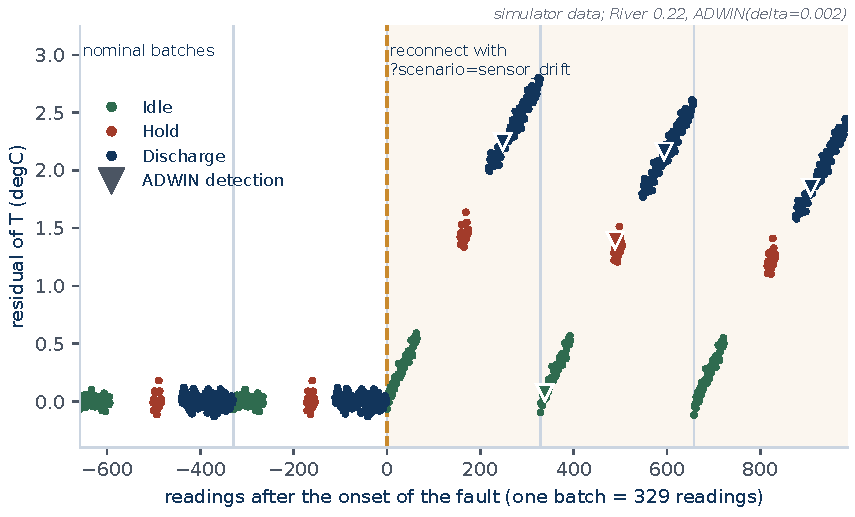
\includegraphics[width=9.2cm]{images/class30_residuals.pdf}};
\foreach \y/\col/\ttl/\txt in {0.1/courseblue/Discharge detects first/{After 248 readings (31\,s live). Its 2--2.5\,°C bias stays in the cooling range: no alert.}, -1.5/coursered/Hold detects last/{After 489 readings: with 19 readings per batch, ADWIN needs a second batch.}, -3.1/coursegold/The baseline absorbs the fault/{The Discharge residual falls from 2.5 to 2.0\,°C in three batches.}} {
  \node[tile, fill=white, draw=\col, thick, anchor=north west, minimum width=3.95cm, minimum height=1.45cm, text width=3.7cm, align=left, font=\scriptsize] at (9.45,\y) {{\bfseries\color{courseblue}\ttl}\\[1pt]\txt};
}
\end{tikzpicture}
\coursefooter
\end{cframe}

\begin{cframe}{Five scenarios, two mechanisms}{\cterm{Coverage gap}{a fault that no rule and no detector of the application can observe.}}
\centering
\begin{tikzpicture}
\foreach \x/\w/\lab in {0/2.7/SCENARIO, 2.85/3.35/{THRESHOLD RULE (HOLD, 72 $\pm$ 1\,°C, 3 READINGS)}, 6.35/3.5/{DRIFT EVENTS (FIRST, READINGS AFTER ONSET)}, 10.0/3.4/DIAGNOSIS} {
  \node[chip, anchor=north west, minimum width=\w cm, minimum height=0.48cm, font=\tiny\bfseries, text width={(\w-0.15)*1cm}, align=center] at (\x,0) {\lab};
}
\foreach \y/\col/\sc/\a/\b/\c in {-0.6/coursegreen/nominal/{none}/{none, no false alarm}/{Normal operation.}, -1.27/coursegold/slow\_heatup/{none}/{none}/{{\bfseries Coverage gap}: needs a HeatUp rule.}, -1.94/coursered/hold\_undershoot/{critical in every batch, first after 159}/{Hold only, after 489}/{{\bfseries Process fault}: one state.}, -2.61/coursegray/sensor\_dropout/{none}/{none; 50 missing readings}/{{\bfseries Data quality}, not drift.}, -3.28/courseblue/sensor\_drift/{critical in every batch, first after 159}/{Discharge 248, Idle 338, Hold 489}/{{\bfseries Sensor fault}: every steady state.}} {
  \node[tile, fill=white, draw=\col, thick, anchor=north west, minimum width=2.7cm, minimum height=0.6cm, font=\ttfamily\scriptsize\bfseries, text=\col!85!black, inner sep=2pt] at (0,\y) {\sc};
  \foreach \x/\w/\t in {2.85/3.35/\a, 6.35/3.5/\b, 10.0/3.4/\c} {
    \node[tile, fill=courseice, anchor=north west, minimum width=\w cm, minimum height=0.6cm, text width={(\w-0.2)*1cm}, align=left, font=\scriptsize, inner sep=2pt] at (\x,\y) {\t};
  }
}
\node[anchor=north west, font=\tiny\itshape, text=coursegray] at (0,-3.95) {Ten nominal batches, then ten batches of the scenario; same monitor as on the previous slides. Reproduce with \texttt{presentations/generate\_class30\_figures.py}.};
\keyidea{-4.3}{Where the drift appears is the diagnosis: in every steady state, the sensor; in one state, the process; nowhere, a gap in coverage.}
\end{tikzpicture}
\coursefooter
\end{cframe}

% ================================================================== PART 3
\sectiondivider{3}{Evolve and close}{sync-alt}{an online baseline and ADWIN detect the sensor fault that the fixed limits miss, and the pattern of detections supports the diagnosis.}{$\bullet$\ The five steps of session 3\\[3pt]$\bullet$\ The design decisions the team must record\\[3pt]$\bullet$\ SRS v3 and one new traceability path}

\begin{cframe}{Session 3: five steps}{\cterm{Test harness}{code that feeds recorded or replayed data to the application and checks its output automatically.}}
\centering
\begin{tikzpicture}
\stepcard{0}{1}{plug}{coursegreen}{Replay and stream}{Add a \texttt{scenario} option; test on \texttt{/replay}, demonstrate on \texttt{/stream}.}
\stepcard{2.71}{2}{graduation-cap}{coursegreen}{Learn the baseline}{One running mean per steady state, test-then-train, with warm-up.}
\stepcard{5.42}{3}{search}{coursegreen}{Detect drift}{One ADWIN per steady state on the residual; record each drift event.}
\stepcard{8.13}{4}{vial}{coursegold}{Run the scenarios}{All five, with a log line, a screenshot, and a test identifier each.}
\stepcard{10.85}{5}{file-signature}{coursegold}{Update the artifacts}{SRS v3, backlog, traceability, operational guide.}
\foreach \x in {2.55,5.26,7.97,10.68} {\draw[arrowgold] (\x,-0.42) -- (\x+0.16,-0.42);}
\keyidea{-4.05}{The thin slice of today: one signal (T), three steady states, one detector type, and the scenario matrix as evidence.}
\end{tikzpicture}
\coursefooter
\end{cframe}

\begin{cframe}{Decisions the team must record}{\cterm{Design decision}{a choice among alternatives, recorded with its rationale so that it can be reviewed.}}
\centering
\begin{tikzpicture}
\infotile{0}{0}{4.35}{1.95}{tilered}{coursered}{lock}{Keep learning or freeze?}{Learning masks the fault; a reset risks the reset loop of Class 29.}
\infotile{4.52}{0}{4.35}{1.95}{tileblue}{courseblue}{sliders-h}{Sensitivity $\delta$}{Smaller $\delta$: fewer false alarms, longer delay. Measure both.}
\infotile{9.05}{0}{4.35}{1.95}{tileblue}{courseblue}{plug}{Reconnection}{A restart loses the baseline: warm up again, or restore it?}
\infotile{0}{-2.1}{4.35}{1.95}{tileblue}{courseblue}{check-double}{Acknowledgement}{Is a drift event acknowledged like an alert? Who closes it?}
\infotile{4.52}{-2.1}{4.35}{1.95}{tilegold}{coursegold}{thermometer-half}{Coverage}{Which rule closes the \texttt{slow\_heatup} gap: final HeatUp T, or dTdt?}
\infotile{9.05}{-2.1}{4.35}{1.95}{tilegreen}{coursegreen}{book-open}{Operator guidance}{What the guide says to do with a drift event, and what not.}
\keyidea{-4.3}{There is no single correct answer: an explicit decision with its rationale and its test evidence is what will be assessed.}
\end{tikzpicture}
\coursefooter
\end{cframe}

\begin{cframe}{SRS v3: one new traceability path}{\cterm{SRS v3}{the specification after the second change request has been analyzed and applied.}}
\centering
\begin{tikzpicture}
\foreach \x/\w/\lab in {0/1.0/ID, 1.16/2.85/REQUIREMENT, 4.17/3.55/ACCEPTANCE CRITERION, 7.88/2.0/IMPLEMENTATION, 10.04/2.0/TEST EVIDENCE, 12.2/1.2/STATUS} {
  \node[chip, anchor=north west, minimum width=\w cm, minimum height=0.4cm, font=\tiny\bfseries] at (\x,0) {\lab};
}
\foreach \x/\w/\txt in {0/1.0/{{\bfseries FR-12}}, 1.16/2.85/{The application shall raise a drift event when the T residual of a steady state changes.}, 4.17/3.55/{After ten nominal batches, \texttt{sensor\_drift} yields a drift event within two batches, with batch, state, signal, detector.}, 7.88/2.0/{Baseline and detector module}, 10.04/2.0/{TC-15: replay log and screenshot}} {
  \node[tile, fill=white, draw=coursegreen!70, thick, anchor=north west, minimum width=\w cm, minimum height=1.95cm, text width={(\w-0.25)*1cm}, align=left, font=\scriptsize, inner sep=3pt] at (\x,-0.5) {\txt};
}
\node[tilegreen, anchor=north west, minimum width=1.2cm, minimum height=1.95cm, font=\scriptsize\bfseries, text=coursegreen] at (12.2,-0.5) {\faIcon{check}\ Passed};
\foreach \x/\w/\txt in {0/1.0/{{\bfseries NFR-06}}, 1.16/2.85/{No drift event shall be raised on the nominal stream.}, 4.17/3.55/{Zero drift events in ten nominal batches after warm-up.}, 7.88/2.0/{Warm-up and $\delta = 0.002$}, 10.04/2.0/{TC-16: replay log}} {
  \node[tile, fill=white, draw=coursegreen!70, thick, anchor=north west, minimum width=\w cm, minimum height=1.15cm, text width={(\w-0.25)*1cm}, align=left, font=\scriptsize, inner sep=3pt] at (\x,-2.6) {\txt};
}
\node[tilegreen, anchor=north west, minimum width=1.2cm, minimum height=1.15cm, font=\scriptsize\bfseries, text=coursegreen] at (12.2,-2.6) {\faIcon{check}\ Passed};
\node[font=\tiny\itshape, text=coursegray, anchor=north west] at (0,-3.8) {example rows: identifiers and test numbers continue the team's own numbering from SRS v2};
\keyidea{-4.2}{A detector needs two acceptance criteria: it detects the fault it is meant for, and it stays silent when nothing has changed.}
\end{tikzpicture}
\coursefooter
\end{cframe}

% ------------------------------------------------------------------ closing
\section{Wrap-up}\gdef\currentsectionname{Wrap-up}
\begin{frame}{From this class to the next}
\centering
\begin{tikzpicture}
\foreach \i/\lab/\bg/\fg in {1/Problem/courseice/coursegray, 2/Data/courseice/coursegray, 3/Features/courseice/coursegray, 4/Model/courseblue/white, 5/Interface/courseice/coursegray, 6/Delivery/courseice/coursegray, 7/Monitor/courseblue/white, 8/Evolution/courseblue/white} {
  \node[rounded corners=3pt, minimum width=1.55cm, minimum height=0.6cm, font=\scriptsize\bfseries, fill=\bg, text=\fg] at ({0.78+(\i-1)*1.68},0) {\lab};
}
\node[font=\tiny\bfseries, text=courseblue] at (6.7,-0.52) {THIS SESSION PUTS AN ONLINE MODEL INSIDE THE MONITORING LOOP};
\foreach \x/\sty/\ico/\ttl/\txt in {0/tileblue/lightbulb/What stays with us/{$\bullet$\ Normal behavior can be learned online.\\[3pt]$\bullet$\ A drift event is evidence for diagnosis, not an alarm.\\[3pt]$\bullet$\ Where drift appears tells what failed.}, 4.55/tileblue/project-diagram/Use it in your project/{$\bullet$\ Test every detector on a replayed fault and on a nominal stream.\\[3pt]$\bullet$\ Decide, and record, what the model does after detection.}, 9.1/tilegold/arrow-right/Next: Classes 31--32/{\textbf{Deployment, serving, Docker, and CI/CD.}\\[3pt]A joint session with a guest lecturer: how an application like yours becomes a reproducible, deployable service.}} {
  \node[\sty, anchor=north west, minimum width=4.3cm, minimum height=3.8cm] at (\x,-0.95) {};
  \badge{\x+0.65}{-1.6}{courseblue}{\ico}
  \node[anchor=west, text width=3.0cm, align=left, font=\small\bfseries, text=courseblue] at (\x+1.2,-1.6) {\ttl};
  \node[anchor=north west, text width=3.9cm, align=left, font=\scriptsize] at (\x+0.2,-2.25) {\txt};
}
\node[tilegold, fill=white, anchor=north west, minimum width=13.4cm, minimum height=0.95cm, text width=12.6cm, align=left, font=\footnotesize] at (0,-5.0) {{\bfseries\goldink\faIcon{route}\ Course thread.} Requirements fix what must hold; online learning keeps track of what is normal; the evidence connects both.};
\end{tikzpicture}
\coursefooter
\end{frame}

% ------------------------------------------------------------------ references
\begin{frame}{Papers and materials}
\centering
\begin{tikzpicture}
\refrow{0}{2.05}{file-alt}{Drift and detection}{Bifet, A. and Gavald\`a, R. (2007). Learning from time-changing data with adaptive windowing. \emph{Proceedings of the SIAM International Conference on Data Mining}, 443--448.\\Gama, J., \v{Z}liobait\.{e}, I., Bifet, A., Pechenizkiy, M., and Bouchachia, A. (2014). A survey on concept drift adaptation. \emph{ACM Computing Surveys}, 46(4), 44:1--44:37.}
\refrow{-2.05}{1.4}{stream}{Streaming learning}{Montiel, J. et al. (2021). River: machine learning for streaming data in Python. \emph{Journal of Machine Learning Research}, 22(110), 1--8.\\Welford, B. P. (1962). Note on a method for calculating corrected sums of squares and products. \emph{Technometrics}, 4(3), 419--420.}
\refrow{-3.45}{1.0}{book}{Documentation}{\href{https://riverml.xyz/latest/api/drift/ADWIN/}{River: \texttt{drift.ADWIN}} and \href{https://riverml.xyz/latest/api/stats/Mean/}{\texttt{stats.Mean}}.\\WHATWG. \href{https://html.spec.whatwg.org/multipage/server-sent-events.html}{HTML Living Standard: Server-sent events}. \ \href{https://docs.streamlit.io/}{Streamlit documentation}.}
\refrow{-4.45}{0.8}{folder-open}{Course materials}{\texttt{documents/Class26\_Pasteurization\_Monitoring\_Challenge.pdf}; \texttt{pasteurization/serving.py}; \texttt{streamlit/pages/App\_Stream.py}.}
\end{tikzpicture}
\coursefooter
\end{frame}

\end{document}
